\section{Discussion}
%
%\subsection{Reduction}
%As it as been mentioned in the introduction, the "abstraction reduction" does not always create smaller abstractions.
%This depends on the type of inputs (discrete, continuous), the number of dimension of inputs, the dimension of the suppressed subspace of the state space and the initial discretization of it.

\subsection{Covering/Overlap in the state space}
When we replace the knowledge of part of the state by the estimation of the state based on inputs, there can be no equivalent discretization of the state space.
Mainly because 2 input sequences can produce reached sets that overlaps.
These overlap (see \ref{fig:overlapp}) cannot happened in discretization of the state space without any memory (the state is supposed to belong to one and only one observation).

We will see later that it can bring to improvement of the size of the abstraction in practice.

\begin{figure}
\centering
\begin{minipage}[b]{0.49\textwidth}
	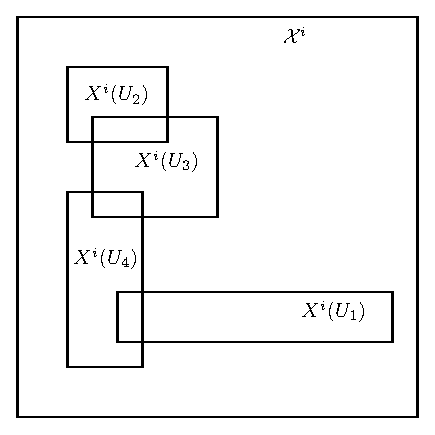
\includegraphics[width=\textwidth]{chapters/abstraction_reduction/overlapp_disc.eps}
\end{minipage}
\caption{The reached sets overlapps. The equivalent discretization of the state space on the left create an abstraction of 7 symbols for 4 symbols in the case of the input extended abstraction.}
\label{fig:overlapp}
\end{figure}


\comment{Self loops -not cool for multi agent task, lose the time information.
Abstractions of asymptotically stable system present a disadvantage on the multiagent control side, for some controls, if the state does not evolve any more, the abstraction will take self loops.
In term multi agent control this make the problem more complex as the control generation: self loops tend to create systems that are asynchronous with all the problems that might occurs because of this (basically one of the agent might be be stopped).}

%size of invariants in the 

%TODO GRAPH TO SHOW IT (I can also do it for the second integrator)

%We will see that in some case it produce smaller abstraction.


\subsection{Reachability}
Reachable sets are computed with the invariant set. As the invariant set is an over approximation of the state, this abstraction is not conservative. This means that for a given problem, it might exist a controller solution for the system $S'$ but no solution for the system $S_a$ (regardless of the memory number).

%\subsection{Notes}
%Self loops are not desirable.
%
%Self loops hide any time information (that is why I have been working on the time information chapter).
%
%In the case of the reduction of the abstraction.

\section{Conclusion}
